\documentclass[lang=cn]{ctexart}
\usepackage{hyperref}
\usepackage{graphicx}
\usepackage{listings}
\usepackage{geometry}
\usepackage{xcolor}
\usepackage{float}
\usepackage{amsmath}

\newtheorem{remark}{注}

\geometry{
    a4paper,
    left=2cm,right=2cm,
    top=2.5cm,bottom=2.5cm
}

\lstset{
	language=lisp,
	basicstyle=\footnotesize\tt,
	numbers=left, numberstyle=\tiny,
	xleftmargin=5em,
	xrightmargin=5em,
	frame=shadowbox,
	backgroundcolor=\color[RGB]{245,245,244},            % 设定背景颜色
	keywordstyle=\color[RGB]{40,40,255},                 % 设定关键字颜色
	numberstyle=\footnotesize\color{darkgray},           % 设定行号格式
	commentstyle=\it\color[RGB]{0,96,96},                % 设置代码注释的格式
	stringstyle=\rmfamily\slshape\color[RGB]{128,0,0},   % 设置字符串格式
	showstringspaces=false,                              % 不显示字符串中的空格
	breaklines=true
}

\title{
    LR(1) 语法分析\footnote{\textit{两次实验的报告和源码都可以在我的\hyperref{https://gitee.com/jerry_yangClover/racket-pascal-mini-cp}{}{}{gitee repo}中找到。}}
    \begin{flushright}\normalsize
        \textit{-- Based on Racket (A Dialect of Lisp)}
    \end{flushright}
}

\author{61519322 杨哲睿}

\begin{document}
\maketitle

\tableofcontents



\newpage

\section{实验要求}

\begin{enumerate}
    \item 手工画出LR(1)项目集族及状态图
    \item 构造LR(1)分析表
    \item 在上述过程中,对二义文法进行必要的处理
    \subitem 表达优先级和结合律
    \subitem 按照优先级和结合律对预测符及状态转换关系进行必要的取舍
    \item 按照LR(1)分析表写出语法分析程序
\end{enumerate}

当然,这只是一个最简单的要求。但考虑到LR(1)分析器的手工构造难度,该实验使用{\heiti 程序推导}的方式来构造LR(1)项目集族和状态转换图。并且在实验的具体实现上有所变化。

\section{设计思路}

根据 \hyperref{https://htdp.org/2021-11-15/Book/part_preface.html#%28part._sec~3asystematic-design%29}{website}{}{htdp} 中的详细介绍,我们可以将设计一个程序分为以下六个步骤:

\begin{enumerate}
    \item From Problem to Data Definitions
    \item Signature, Purpose Statement, Header
    \item Functional Examples
    \item Function Template
    \item Function Definitions
    \item Testing
\end{enumerate}

报告也将从这六个方面展开,对于该语法分析程序的制作进行分析。

\subsection{From Problem to Data Definitions}

\begin{quotation}\textit{
    Identify the information that must be represented and how it is represented in the chosen programming language. Formulate data definitions and illustrate them with examples.}
\end{quotation}

总的来说,我们LR分析程序:
\begin{itemize}
	\item 输入为:Token 的流 (具体实现为\textit{生成器generator})
	\item 输出为:对应的一颗语法树
\end{itemize}

一个LR(1)语法分析程序所涉及的数据结构如下:

\begin{enumerate}
    \item \lstinline|syntax-item| 文法符号 -- 指上下文无关文法中的\textit{非终结符}或\textit{终结符}单元,拥有名称 \lstinline|id|,优先级 \lstinline|proority|、匹配器(函数)\lstinline|matcher|
    \item \lstinline|matched-item| 匹配的文法符号 -- 指输出时匹配后的\textit{终结符}单元
    \item \lstinline|production| 产生式 -- 上下文无关文法的\textit{一个}产生式,分为左部和右部两部分
    \item \lstinline|syntax-tree-node| 语法树的一个节点
    \item \lstinline|LRItem| LR(1) 项 -- 分为四个部分:\textit{产生式的左部、产生式右部在$\cdot$之前的部分、产生式右部在$\cdot$之后的部分、展望(Look-Ahead)符号}
\end{enumerate}

对该数据结构的定义如下:

\begin{lstlisting}[caption={types.rkt}]
(struct syntax-item
 (id priority matcher) #:transparent)
(struct matched-item
 (stx content))
(struct production
 (left right) #:transparent)
(struct syntax-tree-node
 (head children) #:transparent)
\end{lstlisting}

当然这些只是基础的定义,为了完成LR(1)程序,我们还需要定义:

\begin{enumerate}
	\item 一个 LR(1) 项目集就是一个 \lstinline|LRItem| 的\textit{列表}
	\item 一个上下文无关文法包含:\textit{终结符号}、\textit{非终结符号}、\textit{开始符号}、\textit{产生式}
	\item 对于一个增广的上下文无关文法,还需要一个\textit{增广文法的新开始符号}及其对应的\textit{开始符号产生式}
\end{enumerate}

\subsection{Signature, Purpose Statement, Header and Functional Examples}

\begin{quotation}
	\textit{State what kind of data the desired function consumes and produces. Formulate a concise answer to the question what the function computes. Define a stub that lives up to the signature.}
\end{quotation}

根据这些类型的定义,我们足以定义出整个LR(1)语法分析程序的所有函数,如下:

\paragraph{closure}
\begin{description}
	\item[输入] LR(1) 项目集 $I$
	\item[输出] 项目集的闭包 $\mathrm{CLOSURE}(I)$
\end{description}

\begin{remark}
	使用柯里化,这里不需要输入产生式表。
\end{remark}

\paragraph{get-closure-function}
\begin{description}
	\item[输入] 产生式的列表
	\item[输出] $\mathrm{CLOSURE}$ 函数
\end{description}

\begin{remark}
	同理下面几个函数也使用柯里化,降低复杂度。
\end{remark}

\paragraph{get-look-ahead}
\begin{description}
	\item[输入] 产生式列表
	\item[输出] $look-ahead$函数
\end{description}

\paragraph{look-ahead}
\begin{description}
	\item[输入] LRItem
	\item[输出] 当前LRItem在获取到下一个非终结符后的部分的First集
\end{description}
\begin{remark}
	若有 $\mathrm{LRItem}= [A\rightarrow \alpha \cdot B \beta, a]$ 则$look-ahead(\mathrm{LRItem}) = \textsc{FIRST}(\beta)$。这里不需要原来的look-ahead是因为在后续计算中加入了look-ahead的考量。
\end{remark}

\paragraph{go}
\begin{description}
	\item[输入] LR(1)项目集闭包、syntax-item
	\item[输出] 闭包在获取到该syntax-item后产生的新项目集(非闭包)
\end{description}

\paragraph{look-ahead-and-reduce}
\begin{description}
	\item[输入] LR(1)项目集闭包、(读头下的非终结符对应的)syntax-item
	\item[输出] 闭包中可以执行规约的项目列表
\end{description}

\begin{remark}
	这是我实现的方法和书上方法主要的不同:在龙书中,LR自动机的一个项目实则对应了一个项目集(闭包),所以我们无需对于状态进行编号,而只需要通过闭包的转换即可实现等价的自动机行为。这里输出的的可规约的项即为在预测分析表中填上的 $r$,而使用的产生式可以直接通过该规约项所对应的产生式计算得到。
\end{remark}

\begin{remark}
	实际上,我们不需要返回一个列表,因为LR(1)不产生规约-规约冲突。
\end{remark}

\paragraph{try-to-shift-in}
\begin{description}
	\item[输入] LR(1)项目集闭包、(读头下的非终结符对应的)syntax-item
	\item[输出] 闭包中可以执行移进的项目列表
\end{description}


\paragraph{try-to-shift-in}
\begin{description}
	\item[输入] LR(1)项目集闭包、(读头下的非终结符对应的)syntax-item
	\item[输出] 闭包中可以执行移进的项目列表
\end{description}



\paragraph{build-lr1-automata}
\begin{description}
	\item[输入] 产生式列表、增广文法的开始符号的产生式、EOF符号
	\item[输出] 可以在一个token流上执行的自动机
\end{description}

\begin{remark}
	对应于龙书中的LR(1)算法主体,也就是所谓的LR(1)分析的主控。
\end{remark}

\subsubsection{LR自动机}

从实现上说,实际上这不是一个自动机,而是一个先柯里化后的递归函数!

假设我们有一个词法单元(Token,记为$T$)组成的列表 $t_1, t_2, \cdots, t_n, \#$,LR(1)语法分析的输出应该是一颗语法树。简单说即为:

$$
f_1:T\times T\times\cdots \times T \rightarrow \{\mathrm{Syntax~Tree}\}
$$

使用柯里化后:

$$
\begin{aligned}
	f_1:&t_1\mapsto f_2\\
	f_2:&t_2\mapsto f_3\\
	&\cdots\\
	f_n:&t_n \mapsto f_{n+1}\\
	f_{n+1}:&\# \mapsto \mathrm{Syntax~Tree}
\end{aligned}
$$

可以看出,其输入都是相同的,而提供给函数的实际上是一个流对象(生成器),所以考虑最后将其转换为递归函数实现。在实验1中,已经说明了:状态机的实质就是从函数和输入到另一个函数的映射(状态转换函数)。因此,在语法分析实现过程中,将LR自动机实现为这样的函数。但实现中不难发现一个问题,由于我们在编码时无法确定状态总数,状态转换函数都定义为匿名函数。也就是说,这个递归函数跳转时跳转的对象是没有事先绑定的,显然,这是一个Y-组合子问题。

当然,我们也可以做出一点改变,用一个很不函数式的方法来实现类似于一个Y-组合子的方法,我们将每一个状态及其对应的状态转换函数,写入一个哈希表中,在进行状态跳转的同时在哈希表里面查询相应的表项执行,来避免Y-组合子中无法进行匿名函数变量绑定的问题。

\subsection{Function Template}\label{Function-Template}
\begin{quotation}
	\textit{Translate the data definitions into an outline of the function.}
\end{quotation}

在\ref{Function-Template}中,仅仅给出 \lstinline|build-lr1-automata| 的定义过程,因为该函数足以诠释整个算法的构造流程。

\subsubsection{LR(1)自动机构造基础}

给定产生式列表、增广文法的开始符号产生式,我们可以计算如下内容:

\begin{enumerate}
	\item $\mathrm{CLOSURE}$ 函数(Currying)
	\item $I_0$:即自动机的初始状态所对应的项集闭包
	\item $\mathrm{GOTO}$ 函数
\end{enumerate}

\begin{remark}
	在这里的 $\mathrm{GOTO}$ 函数和先前定义的 $\mathrm{GO}$ 函数是不同的,GO函数仅仅计算出从闭包 $I_1$ 通过输入文法符号 $A$ 得到的下一个闭包 $I_2$,但在这里,$I_2$ 是通过$I_1$推导的,虽然本质上重复两次计算 $\mathrm{GO}(I_1, A)$ 所得到的 $I_2$ 是相同的(函数是单值映射),但在计算机内部,由于通过了两次推导,用面向对象的说法即是两个截然不同的对象。
\end{remark}

注意,上面实现的 $\mathrm{GOTO}$ 函数是可以接受终结符号的!在报告实现的语法分析器中,由于将自动机的状态和LR(1)项目集构建了一一对应关系,即自动机运行时能确定自身状态对应的LR(1)项目集,可以通过该项目集和输入的符号和$\mathrm{GOTO}$函数来确定执行移进或者规约。换言之,不需要用 $\mathrm{ACTION}$ 函数即可实现该自动机。实现如下:考虑原有的移进和规约的执行逻辑,
	
在LR(1)分析表中填入移进,当下面两项中有且仅有一项成立:

\begin{enumerate}
	\item $\mathrm{GO}(I_1, a) = I_2$ 且 $a$ 是终结符号,那么在 $\mathrm{ACTION}$ 中填入移进并且转状态 $I_2$(项目集对应的状态)
	\item $\mathrm{GO}(I_1, A) = I_2$ 且 $A$ 是非终结符号,那么在 $\mathrm{GOTO}$ 中填入状态 $I_2$
\end{enumerate}

重点关注非终结符号情况:在LR自动机执行的过程中,\textbf{必定是在规约得到了一个非终结符号后执行}$\mathrm{GOTO}$\textbf{操作}。对于这类情况我们可以简单的执行如下三个内容:把\textit{读头}下的内容转换为该非终结符号,并重新执行移进所对应的逻辑即可。

\subsubsection{LR(1)预测分析程序}

这样的设计是合理的,我们可以设置这样的函数参数 \lstinline|buf|,作为''移入''的符号。读头下的 \lstinline|token| 它一定和某一个终结符匹配,那么转换为一个\lstinline|matched-item|,其中的\lstinline|stx|属性是其匹配的终结符,\lstinline|content|对应该\lstinline|token|。考虑两种情况:
\begin{enumerate}
	\item 移入:程序在token流中取出下一个token,并作为下一状态转换函数的 \lstinline|buf| 参数传入。
	\item 规约:\lstinline|buf| 的符号需要保存(作为返回值传递给上一层递归函数调用),所以我们在规约前后都需要保存当前读头下的非终结符。
	
	在规约完后,该函数会返回\lstinline|buf|和一颗语法树。(这相当于原来LR分析主控算法中的使用某个产生式来执行规约)然后我们对于拿到的语法树的头部非终结符执行移进(相当于按照分析表,执行GOTO部分),并将原\lstinline|buf|中的词法单元执行传给该状态转换函数尝试进行下一步的状态转换。
\end{enumerate}

具体实现请见 \ref{source-build}

\subsubsection{优先级判断}

不难发现,我们设计的二义文法在优先级上体现为移进-规约冲突,这可以通过:
\begin{itemize}
	\item 规约的LR1项的产生式右部在 $\cdot$ 之前的部分的最后一个终结符
	\item 移进的LR1项的移进符号(实际上就是读头下的符号)
\end{itemize}
的优先级来判断!

考虑移进规约冲突如下:
$$
(E\rightarrow E+E\cdot, \times)\quad(E\rightarrow E \cdot \times E, +)
$$

由于规约项中的 $\times$ 比 $+$ 优先级高,所以执行移进。其余情况同理处理。

\subsection{Function Definition}
\begin{quotation}
\textit{Fill in the gaps in the function template. Exploit the purpose statement and the examples.}
\end{quotation}

这里就不多进行函数定义的解释了,具体实现方法可以在\ref{source}找到。

\section{算法测试}

\begin{quotation}
	\textit{Articulate the examples as tests and ensure that the function passes all. Doing so discovers mistakes. Tests also supplement examples in that they help others read and understand the definition when the need arises—and it will arise for any serious program.}
\end{quotation}

我们用龙书的例 4.54 作为测试用例:

\lstinputlisting{../syntax/test3.rkt}

该测试用例产生了输出:

\lstinputlisting{../syntax/result4.txt}

\begin{remark}
	前几行是从产生式中推断所有的非终结符的First集,然后得到了所有的终结符号,继而通过不动点算法迭代产生所有的闭包。最后通过自动机来实现语法分析。
\end{remark}

通过最后一行的输出,放在Mathematica中进行图形化:

\begin{figure}[H]
	\centering
	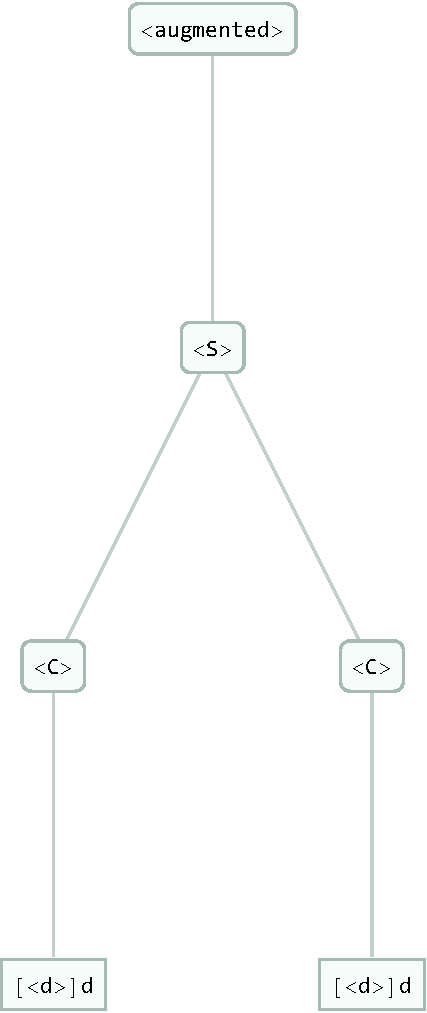
\includegraphics[width=0.2\linewidth]{pic/dd}
	\caption{对于dd的分析结果}
	\label{fig:dd}
\end{figure}


我们将原来的测试字符串替换为:\lstinline|cdccd|,那么

\begin{figure}[H]
	\centering
	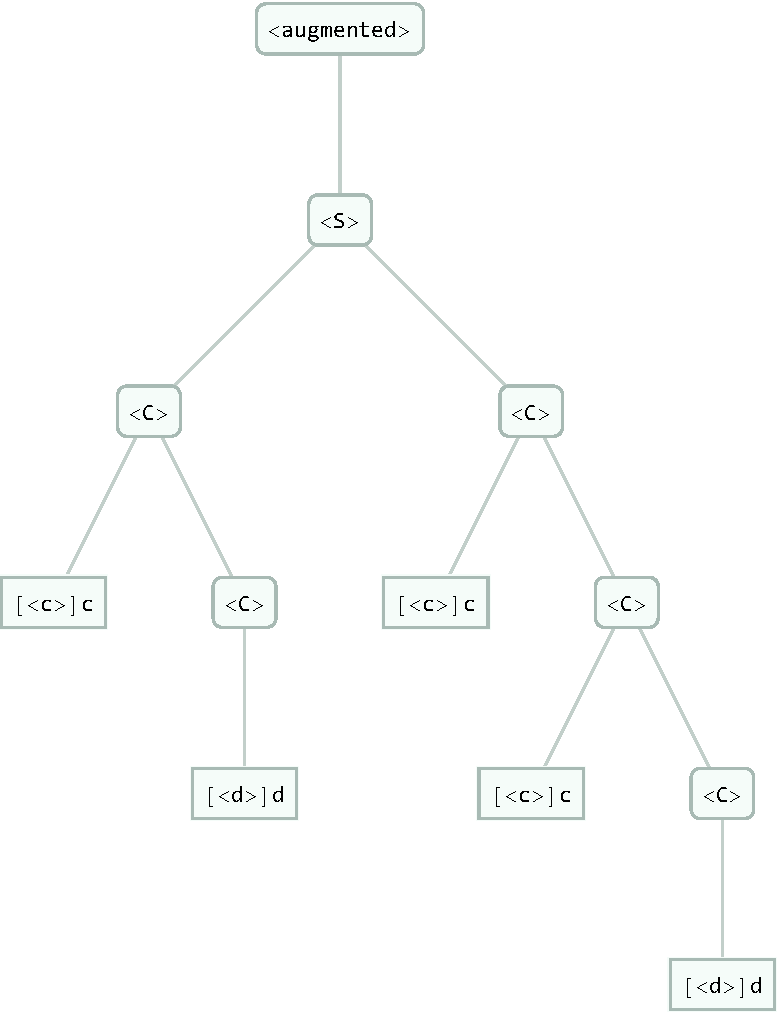
\includegraphics[width=0.5\linewidth]{pic/cdccd}
	\caption{cdccd的分析结果}
	\label{fig:cdccd}
\end{figure}

当然,我们写出如下的产生式:
\begin{lstlisting}
(define productions
 (list
  (production STX-FAKE-S (list STX-EXPR))
  (production STX-EXPR (list stx-sep-lbracket STX-EXPR stx-sep-rbracket))
  (production STX-EXPR (list STX-EXPR stx-relop-plus STX-EXPR))
  (production STX-EXPR (list STX-EXPR stx-relop-minus STX-EXPR))
  (production STX-EXPR (list STX-EXPR stx-relop-divide STX-EXPR))
  (production STX-EXPR (list STX-EXPR stx-relop-assign STX-EXPR))
  (production STX-EXPR (list STX-EXPR stx-relop-multi STX-EXPR))
  (production STX-EXPR (list stx-number))
  (production STX-EXPR (list stx-identifier))))
\end{lstlisting}

$$
1 - 2 + 3 * 4 - 5 / 6 + (7 + 8) * 9
$$
也可以简单的对于下述表达式进行语法分析:
\begin{figure}[H]
	\centering
	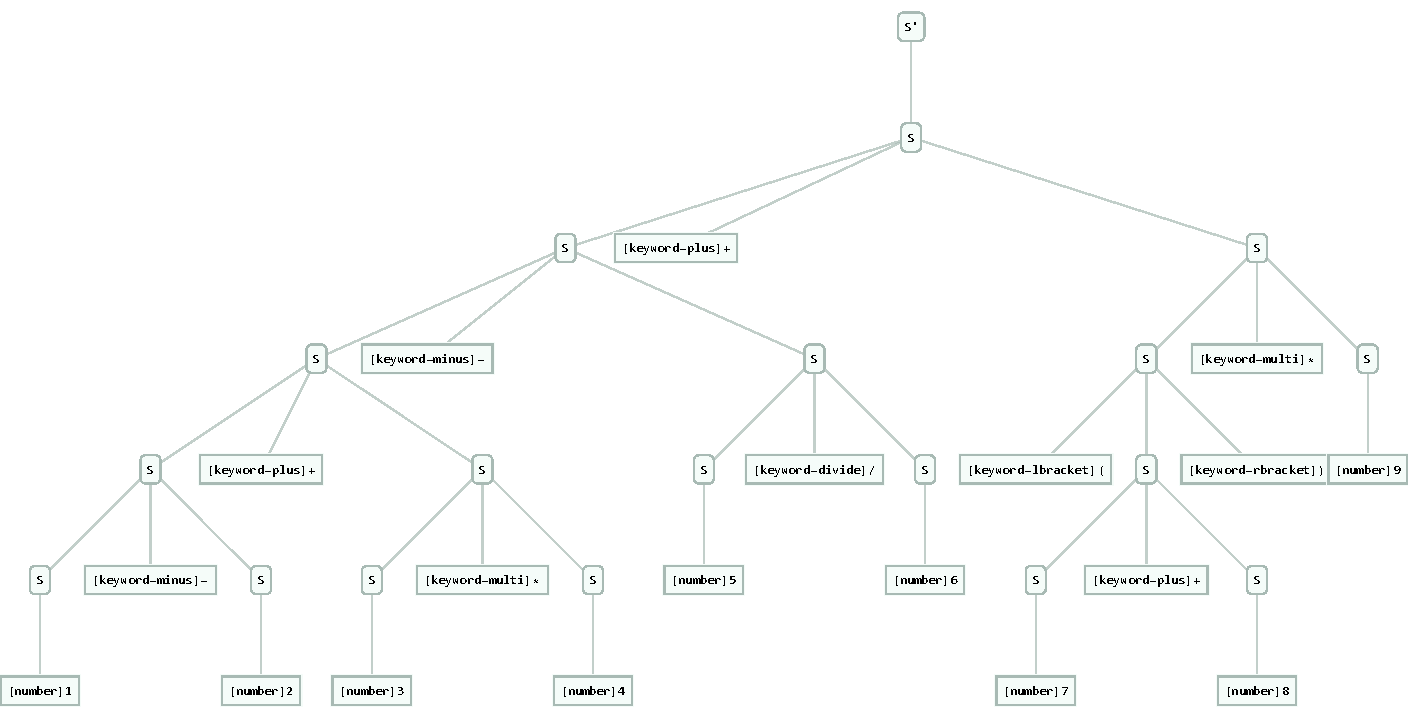
\includegraphics[width=0.7\linewidth]{pic/expr}
	\caption{上述表达式的语法树。可以看出,正确的进行了 * 、 + 、()的优先级判断.}
	\label{fig:expr}
\end{figure}

当然也可以对下述程序进行分析:(产生式在:\ref{source-main})
\lstinputlisting[language=pascal]{../syntax/test2.pas}

\begin{figure}[H]
	\centering
	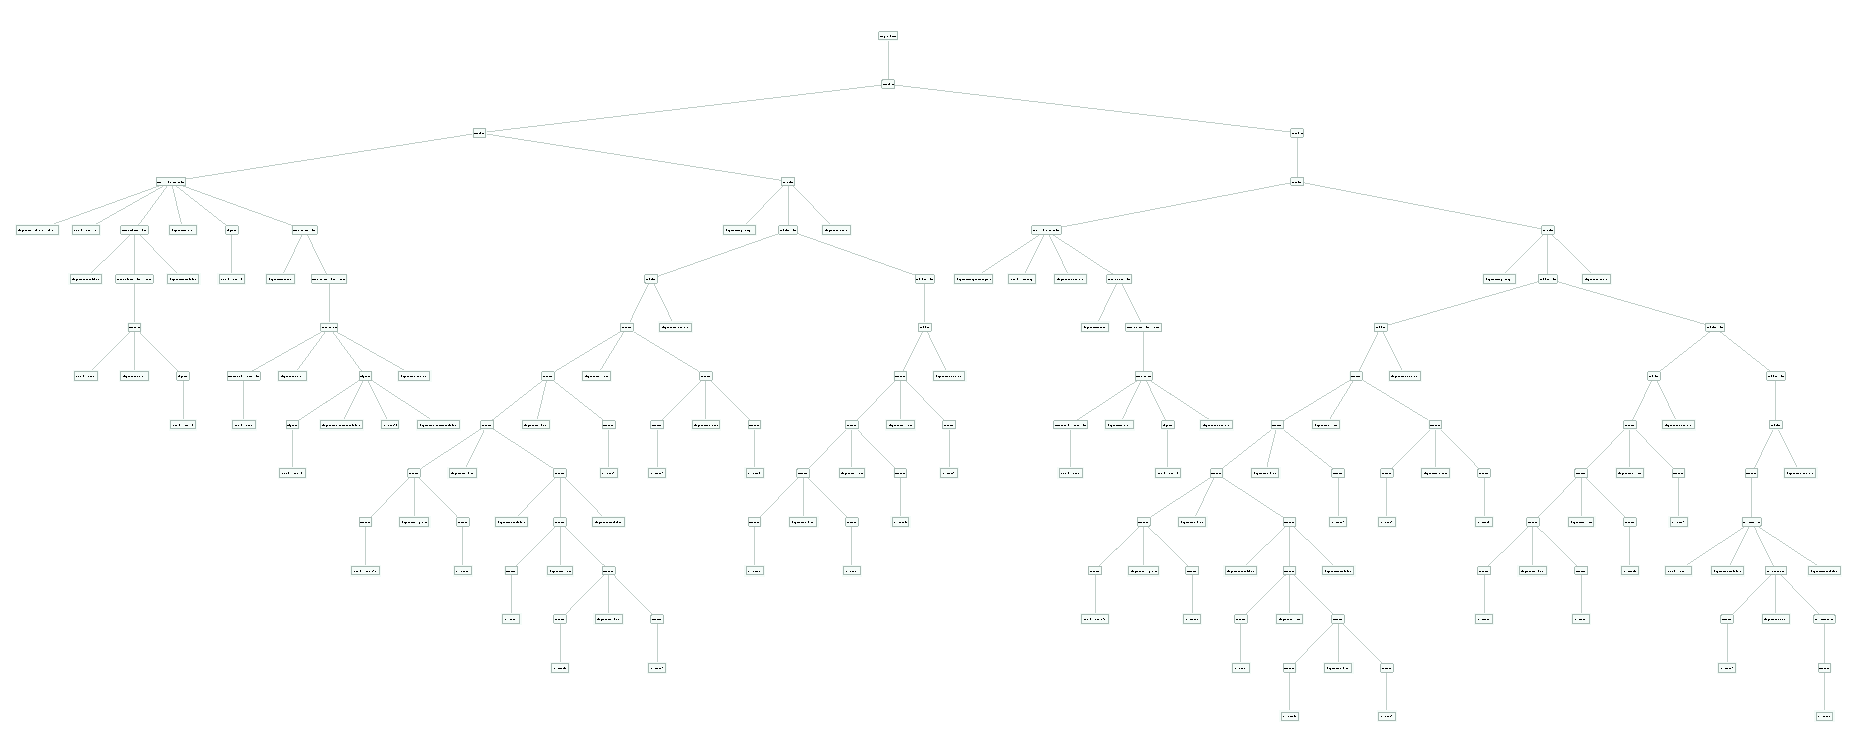
\includegraphics[width=0.7\linewidth]{pic/a-large-program}
	\caption{上述程序的语法分析结果}
	\label{fig:a-large-program}
\end{figure}

\begin{remark}
	这个放大应该能看清楚吧。(毕竟是pdf导出的嘿嘿) :)
\end{remark}

\section{总结}

{\tiny 妈的},终于调通了!总的来说,实验对于书上各个算法进行一些等价变换,然后给出了函数签名,阐述函数作用,最终完成这样的一个算法实现。当然中间Debug真的很复杂,因为要将状态转换表和LR(1)项集在脑子里面不断地转换,将reduce操作的退栈过程等价到函数调用返回时的返回、退栈操作,把$\mathrm{GOTO}$和$\mathrm{ACTION}$整合,并实现原有的功能,最终实现了LR(1) 的自动推导、和自动机分析,能够配合原有的词法分析器实现对于简单 Pascal 源码的词法、语法分析,产生对应的语法树。

\section{源码}\label{source}

两次实验的报告和源码都可以在我的\hyperref{https://gitee.com/jerry_yangClover/racket-pascal-mini-cp}{}{}{gitee repo}中找到。

\subsection{build-lr1-automata}\label{source-build}

\lstinputlisting[basicstyle=\footnotesize\ttfamily,breaklines=true,caption={build.rkt}]{../syntax/build.rkt}

\subsection{Pascal 产生式定义}\label{source-main}

\lstinputlisting[caption={main.rkt}]{../syntax/main.rkt}

\end{document}











